% !TeX root = ../../main.tex
\section{Introduction}

This report explains the design for the separation of p-nitrotoluene (PNT) from a liquid stream consisting predominantly of PNT and m-nitrotoluene (MNT) with a trace of o-nitrotoluene (ONT). Since the production of 4-ABH and 4-ABA requires PNT as the precursor with at least 90\% purity, this separation must be carefully considered and designed. Table \ref{tab:inlet crystalliser} summarises the inlet conditions for this separation. 

\begin{table}[h] \label{tab:inlet crystalliser}
\centering
\caption{Inlet conditions for the separator unit to be designed in details.}
\begin{tabular}{@{}l|l|l|l|l|l@{}}
\toprule
\textbf{Total mass flowrate (kg/s)}  & \textbf{Temperature (K)}  & \textbf{Pressure (atm)} & \textbf{MNT (kg/kg)} & \textbf{ONT (kg/kg)} & \textbf{PNT (kg/kg)}   \\ \midrule
0.0395  & 331 &  1 & 0.1092 & 0.0069  &   0.8839 \\ \bottomrule
\end{tabular}
\end{table}

A system consisting of a melt crystalliser and a hydraulic wash column has been chosen as appropriate separators. Both units were modelled to determine appropriate dimensions and evaluate the performance of the units. A sensitivity analysis has been conducted on variables with uncertainty to demonstrate its effect on the designs and the output. Finally, mechanical designs with supplementary CAD drawings of both units are included.


\begin{figure}[h]
    \centering
    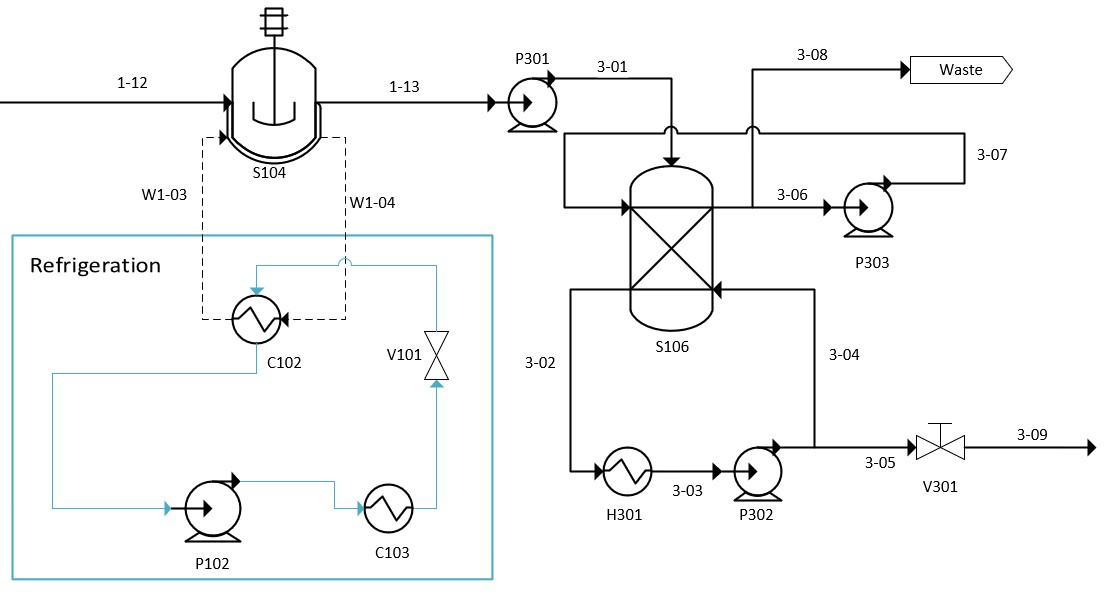
\includegraphics[scale=0.5]{chapters/3-separation/figures/Crystallizer PFD.jpg}
    \caption{PFD of the separation system in consideration}
    \label{fig:crystalliser schematic}
\end{figure}

